\chapter{Diseño}
 En este capítulo nos centraremos en el diseño elegido después de haber analizado los requisitos de nuestro sistema. De aquí obtendremos la estructura de base de datos idónea para un correcto desarrollo del aplicativo, además de la arquitectura necesaria para llevar a cabo todos estos procesos.
 
\section{Base de datos}

El sistema puede ser diferenciado en 4 grandes bloques.

Por una parte tenemos a los usuarios. Estos pueden tener varios roles como son los clientes, los trabajadores y los superadministradores. Todos podrán interactuar con las funcionalidades (según su rol)  proporcionadas por el web service a los dominios Front-End de cada negocio, sin embargo el rol diferenciador entra en juego en la parte de administración de negocios y el propio sistema mencionado. Un usuario deberá estar ligado a un único negocio, ya que, aunque la información se almacenen en la misma base de datos el usuario final no tiene por qué saber que negocios pertenecen al sistema.

Por otra parte tenemos los negocios, que, para que todo tenga sentido, el sistema permita una rápida implementación de nuevos clientes, donde se crearán configuraciones para las distintas secciones. De esta forma, aunque se separen el Front-End del Back-End, podremos configurar y personalizar nuestra web de la forma que deseemos (dentro de lo permitido por la configuración implementada). Sin olvidar la configuración de horarios, tiempos entre cita y cita, etc.

Las citas son también uno de los bloques principales de este sistema. Se deberá guardar información relevante a la cita, la cual deberá estar asignada a un usuario y a un trabajador del negocio determinado. Guardar datos referentes a la fecha de registro de la cita puede ser interesante de cara al análisis estadístico de los negocios que lo deseen.

Por último, pero no menos importante tenemos la parte de la venta de productos online. Esto conlleva el registro de productos para el negocio y de pedidos para los clientes que deseen acceder a este servicio. Un producto deberá estar asociado a un negocio, un pedido deberá tener uno o muchos productos además de estar asociado a un único usuario. No podemos olvidar que para realizar el envío de los pedidos realizados el usuario deberá indicar una dirección. Consecuentemente añadiremos una entidad de direcciones que se relacionará con el usuario de forma que un usuario pueda tener cero o más direcciones y una dirección pueda pertenecer a uno o varios usuarios.

Vamos ahora por tanto a representar el diagrama de Entidad-Relación: 

\begin{figure}[H]
  \centering
  \includegraphics[scale=0.25]{images/Diagrama_Entidad_Relación_Refactor.png}
  \caption{Diagrama Entidad-Relación}
  \label{}
\end{figure}

\subsection{Paso a tablas y fusión}

Una vez definido nuestro esquema Entidad-Relación procedemos al paso a tabla y la fusión de las mismas. Primero definiremos las tablas de las entidades del sistema junto con sus relaciones (1-12). En la fusión de las anteriores tablas podemos encontrar la unión de las citas previas (appointment) junto con los trabajadores y clientes que atienden y reciben estas citas respectivamente, quedando así una tabla con todos los datos respectivos a una cita. Ocurre lo mismo con la tabla de pedidos y sus relaciones, ya que uniendo 4-9-11 conseguimos aunar la información del usuario, a donde va dirigido y los datos relativos al mismo como son el estado, el precio, la fecha, etc.

% \begin{figure}[H]
%   \centering
%   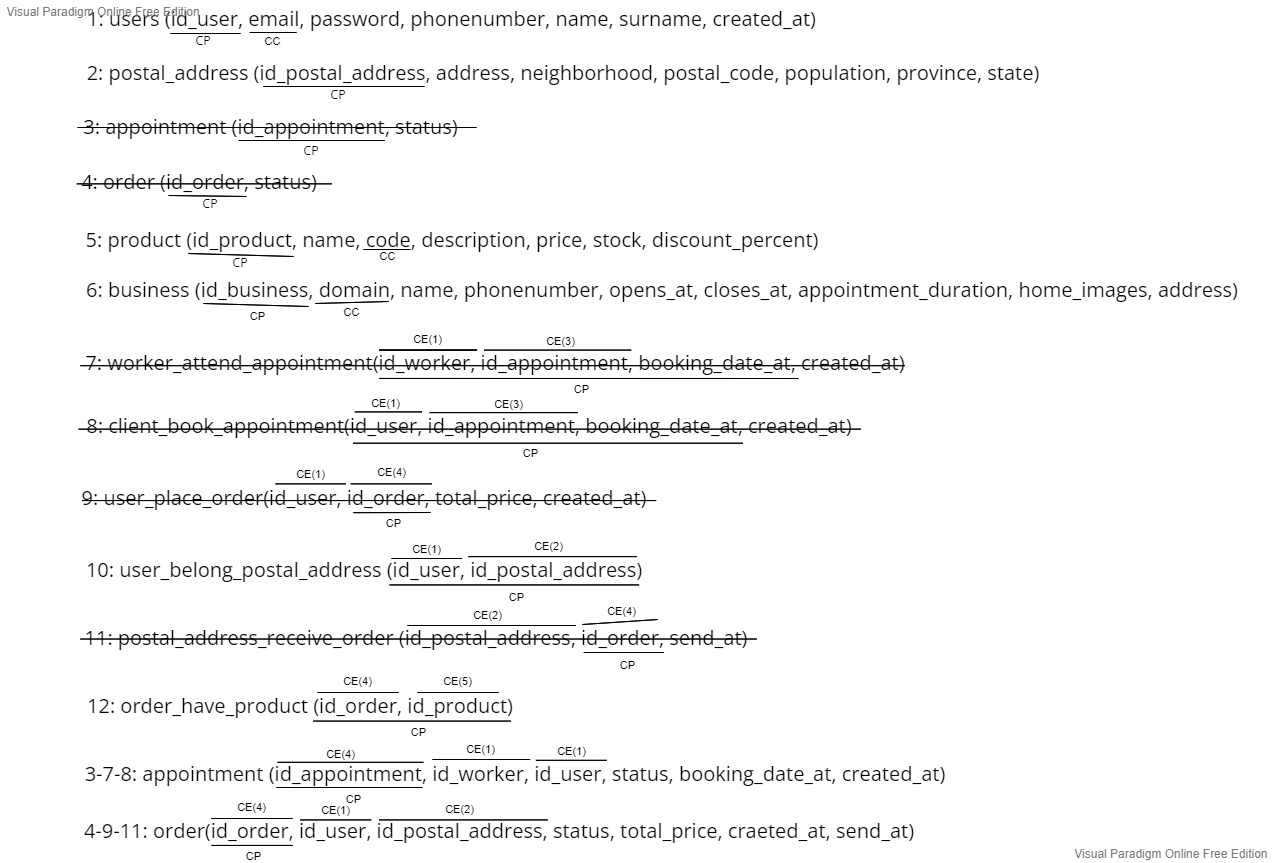
\includegraphics[scale=0.3]{images/Paso_a_Tablas.png}
%   \caption{Paso a tablas y fusión}
%   \label{}
% \end{figure}

Por último para la agregación del negocio con las respectivas entidades y relaciones, se añadirá un ID identificativo de la tienda que relacione a esta con cada una de las tablas que son almacenadas en el sistema.

\begin{figure}[H]
  \centering
  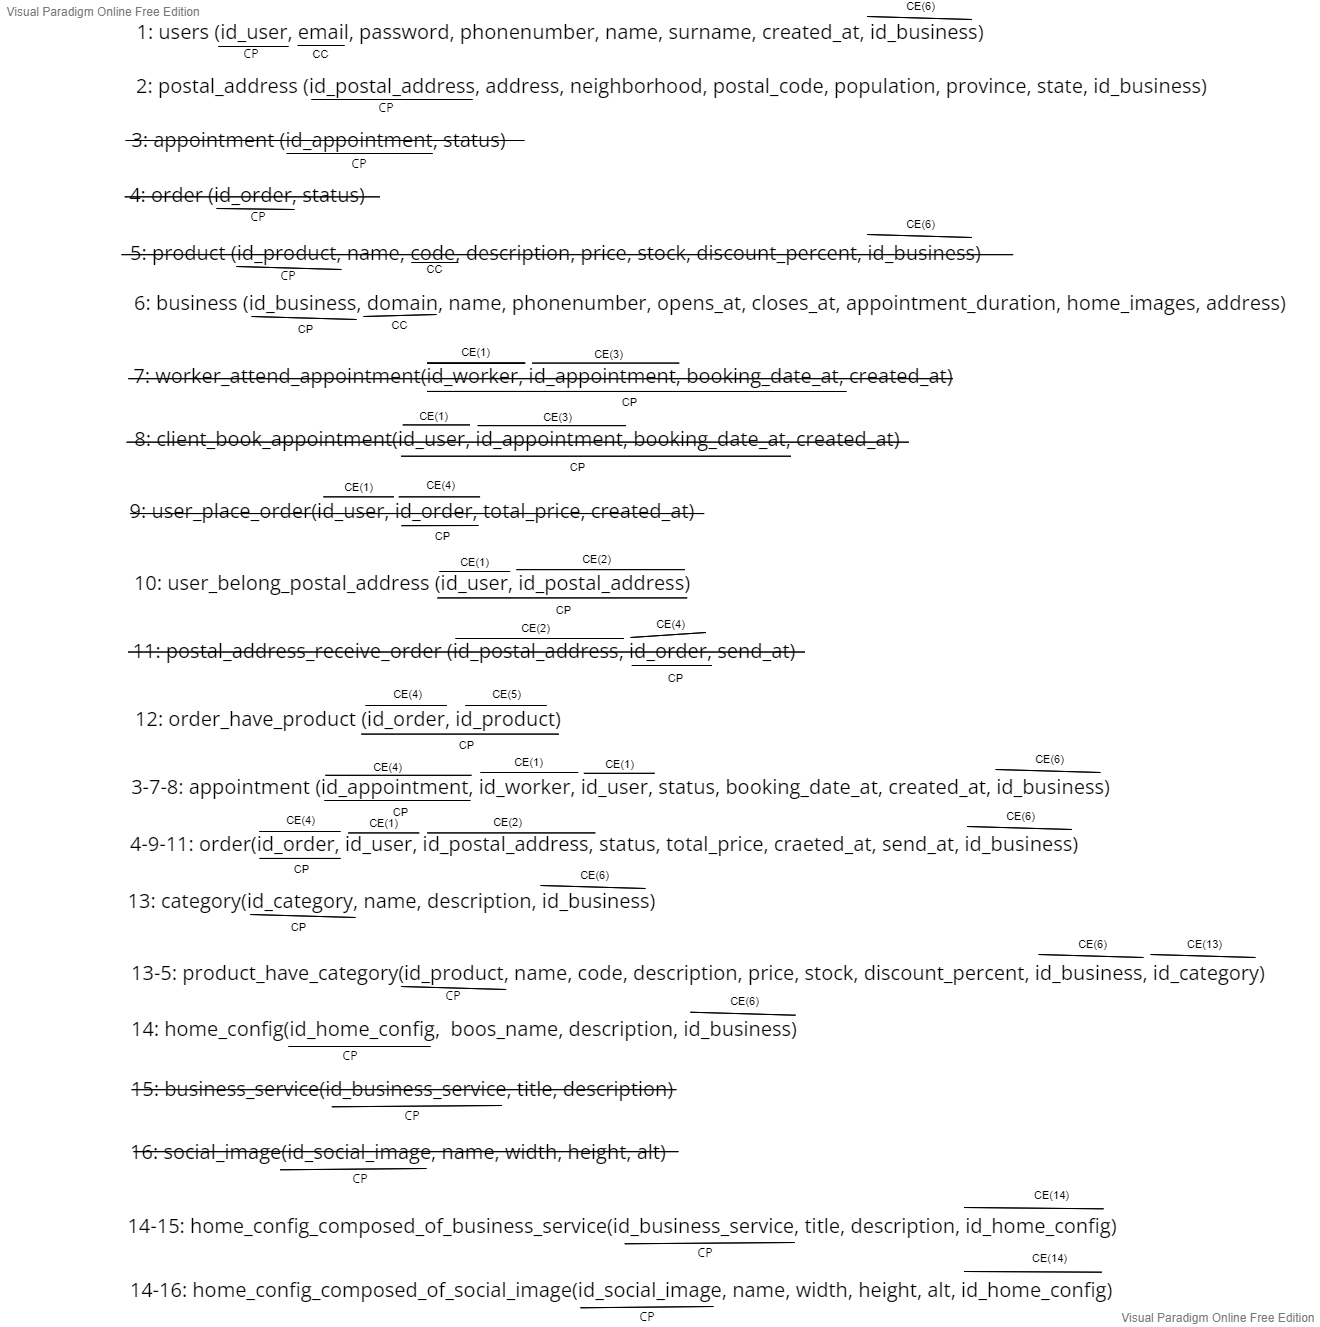
\includegraphics[scale=0.3]{images/Paso_a_Tablas_Negocio_Refactor.png}
  \caption{Paso a tablas y fusión}
  \label{}
\end{figure}

\subsection{Normalización}

El proceso de normalización es un proceso de descomposición de los esquemas de relación hasta que
todas las relaciones alcancen la forma normal deseada.\cite{normalizacion} Analizaremos por tantos las diferentes Formas Normales:

\vspace{-0.5em}
\begin{itemize}
    \item \textbf{Primera Forma Normal (1FN)}: Una relación está en primera forma normal cuando todos sus atributos son atómicos.\cite{1fn} Como se observa nuestra base de datos ya se encuentra en la Primera Forma Normal, ya que cumple con todos los requisitos: sus atributos son atómicos, las tablas contienen una clave primaria única y sin atributos nulos, existe independencia con el orden de filas y columnas.

    \item \textbf{Segunda Forma Normal (2FN)}: Una relación está en 2FN si está en 1FN y si los atributos que no forman parte de ninguna clave dependen de forma completa de la clave principal. Es decir que no existen dependencias parciales. (Todos los atributos que no son clave principal deben depender únicamente de la clave principal).\cite{2fn} Podemos afirmar también que nuestras tablas se encuentra en Segunda Forma Normal debido a la dependencia completamente funcional entre los campos de las mismas.

    \item \textbf{Tercera Forma Normal (3FN)}: La tabla se encuentra en 3FN si es 2FN y si no existe ninguna dependencia funcional transitiva entre los atributos que no son clave.\cite{3fn} Por consecuente nuestra base de datos se encuentra en Tercera Forma Normal, ya que no presenta relaciones transitivas (no hay tablas que presenten ningún campo no clave dependiente de ningún otro campo no clave).
\end{itemize}

\section{Arquitectura del Sistema}

Como se ha indicado ya en varios puntos de esta documentación nuestro sistema estará separado en Front-End y Back-End. Aún así el diseño de la arquitectura se basa en el clásico Modelo-Vista-Controlador (MVC) pero dividiéndolo en lo que podríamos llamar módulos.

Por una parte el Web Service implementado será nuestro Modelo-Controlador, que será el encargado de manejar los datos del aplicativo y devolverlos o procesarlos a través de los controladores a los solicitantes. La vista se separa del modelo controlador por cada una de las páginas webs que estén integradas en el sistema, por lo que no habrá únicamente una vista, habrá múltiples vistas que haga uso de la arquitectura de Back-End del Modelo-Controlador.

A su vez en la parte Back-End se implementará una administración para los trabajadores del negocio completando así un nuevo MVC para la gestión de los datos almacenados.

\begin{figure}[H]
  \centering
  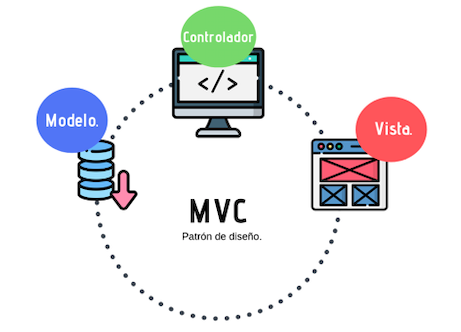
\includegraphics[scale=0.6]{images/Modelo_Vista_Controlador.png}
  \caption{Modelo Vista Controlador}
  \label{}
\end{figure}

\section{Interfaz de Usuario}

Previo al comienzo de la implementación y desarrollo de la aplicación esbozaremos unos bocetos de como será la interfaz con la que tengan que interactuar los usuarios de los negocios que se encuentren en el sistema. Un diseño de interfaz \cite{design} puede marcar la diferencia a la hora de las conversiones para el negocio. Por ejemplo, un diseño demasiado complejo o poco llamativo para una tienda online puede hacer que sus ventas bajen considerablemente.

Vamos a definir por tanto los diseños de las páginas principales de los negocios del sistema.

\subsection{Página de Inicio}

Esta será la página principal del negocio. En ella podremos encontrar diferentes secciones con información relativa a este (descripciones del funcionamiento del negocio, de los trabajadores, imágenes de las tareas desempeñadas en el negocio, etc.). Se pretende que el diseño sea llamativo y moderno para que llame la atención del usuario y decida seguir navegando por la web.

Contendrá también una barra de navegación, que acompañará en todas las páginas como podremos ver, y un footer con información importante como puede ser la dirección, teléfono o datos de contacto del personal del negocio.

\begin{figure}[H]
  \centering
  \includegraphics[scale=0.6]{images/Diseño_Pag_Inicio.png}
  \caption{Página de Inicio de Web}
  \label{}
\end{figure}

\subsection{Página de Tienda}

La página de Tienda tendrá un formato sencillo y simple. Como hemos indicado, una web demasiado compleja puede llevar a un bajo nivel de tráfico. En un lateral encontraremos la sección de filtros para los productos y en la parte principal encontraremos los productos paginados. La paginación es importante debido a que evitará que el usuario tenga que hacer un scroll desmesurado para encontrar el producto deseado.

\begin{figure}[H]
  \centering
  \includegraphics[scale=0.6]{images/Diseño_Pag_Shop.png}
  \caption{Página de Tienda de Web}
  \label{}
\end{figure}

\begin{figure}[H]
  \centering
  \includegraphics[scale=0.5]{images/Diseño_Pag_Shop_Carrito.png}
  \caption{Página de Tienda de Web con Carrito de Compra}
  \label{}
\end{figure}

\subsection{Página de Reserva de Citas}

Al igual que en la página de Tienda, se implementará un diseño simple e intuitivo para la reserva de citas del negocio.
En la página podremos ver un calendario, el cual podremos elegir el mes en el que situarnos, y los días del mes marcados con colores en los que el usuario pueda apreciar si el día está disponible o no para reservar una cita sin necesidad de acceder a él.

Al acceder a un día deseado por el usuario podremos ver un Popup similar al de carrito de compra que nos indicará el día seleccionado y las citas disponibles de las que disponemos según el turno de trabajo (mañana o tarde).

\begin{figure}[H]
  \centering
  \includegraphics[scale=0.6]{images/Diseño_Pag_Appointment.png}
  \caption{Página de Reserva de Citas de Web}
  \label{}
\end{figure}

\begin{figure}[H]
  \centering
  \includegraphics[scale=0.5]{images/Diseño_Pag_Appointment_Dia.png}
  \caption{Página de Reserva de Citas (selección de día)}
  \label{}
\end{figure}

\subsection{Página de Perfil de Usuario}

Por último vamos a mostrar el diseño de la página de Perfil de Usuario. En esta podremos ver 3 secciones relativas a toda la información relacionada con los perfiles de los clientes como son los datos personales, las citas reservadas y los pedidos realizados. Las maquetaciones serán sencillas y sin demasiada carga visual para el cliente (dentro de lo posible para mostrar la información importante).

\begin{figure}[H]
  \centering
  \includegraphics[scale=0.5]{images/Diseño_Pag_User_Datos.png}
  \caption{Página de Perfil de Usuario (datos personales)}
  \label{}
\end{figure}

\begin{figure}[H]
  \centering
  \includegraphics[scale=0.5]{images/Diseño_Pag_User_Citas.png}
  \caption{Página de Perfil de Usuario (citas)}
  \label{}
\end{figure}

\begin{figure}[H]
  \centering
  \includegraphics[scale=0.5]{images/Diseño_Pag_User_Pedidos.png}
  \caption{Página de Perfil de Usuario (pedidos)}
  \label{}
\end{figure}

\begin{figure}[H]
  \centering
  \includegraphics[scale=0.5]{images/Diseño_Pag_User_Pedidos_Popup.png}
  \caption{Página de Perfil de Usuario (datos de pedido)}
  \label{}
\end{figure}